\section{Teilaufgabe 3}
\begin{aufgabe}
    Programmieren Sie diese 2 Übertragungsfunktionen im gleichen Simulink 
    Diagramm (wo Sie den Wirkungsplan programmiert haben) und führen Sie die 
    gleichen Simulationen wie vorher durch. Prüfen Sie die Plausibilität der 
    Ergebnisse und passen Sie darauf auf, dass Wirkungsplan und 
    Übertragungsfunktionen die gleichen Ergebnisse liefern (wenn die 
    Anfangsbedingung für die Drehzahl gleich null ist). Ab diesem Punkt wird 
    nur mit den Übertragungsfunktionen gearbeitet.
\end{aufgabe}
\begin{figure}[h!]
    \centering
    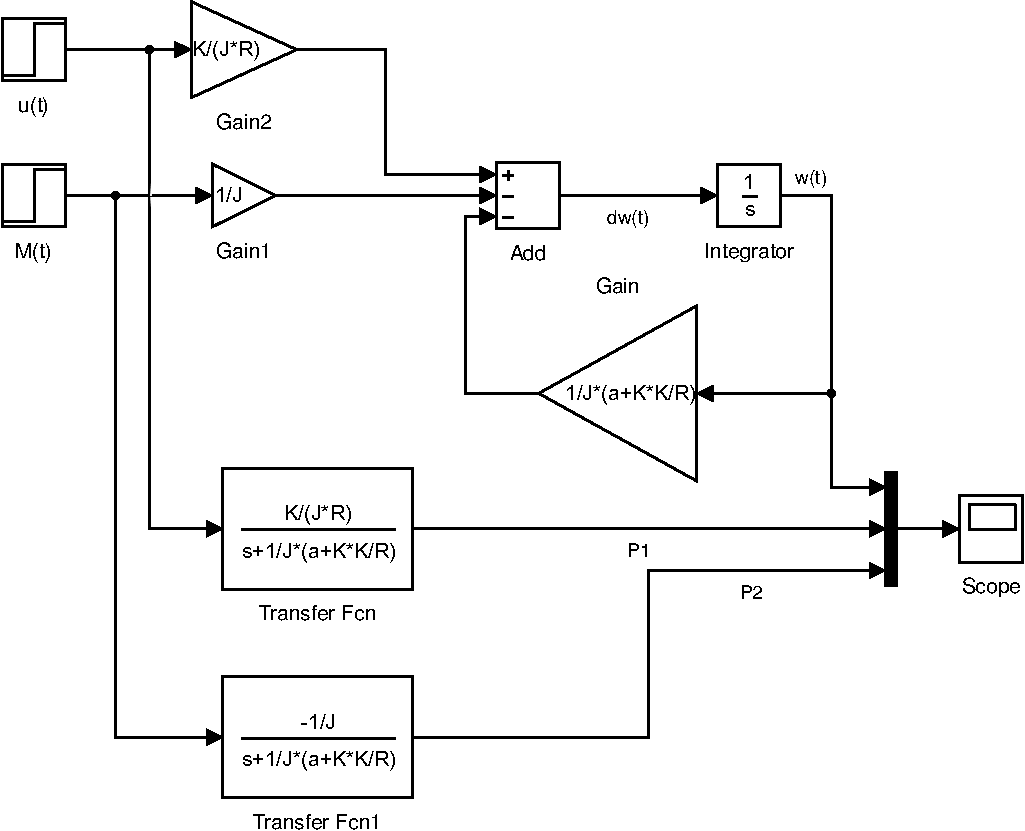
\includegraphics[width=0.6\textwidth]{03/transfer.pdf}
    \caption{Übertragungsfunktionen $P_1$ und $P_2$ in Simulink}
    \label{fig:03}
\end{figure}
\begin{figure}[h!]
    \centering
    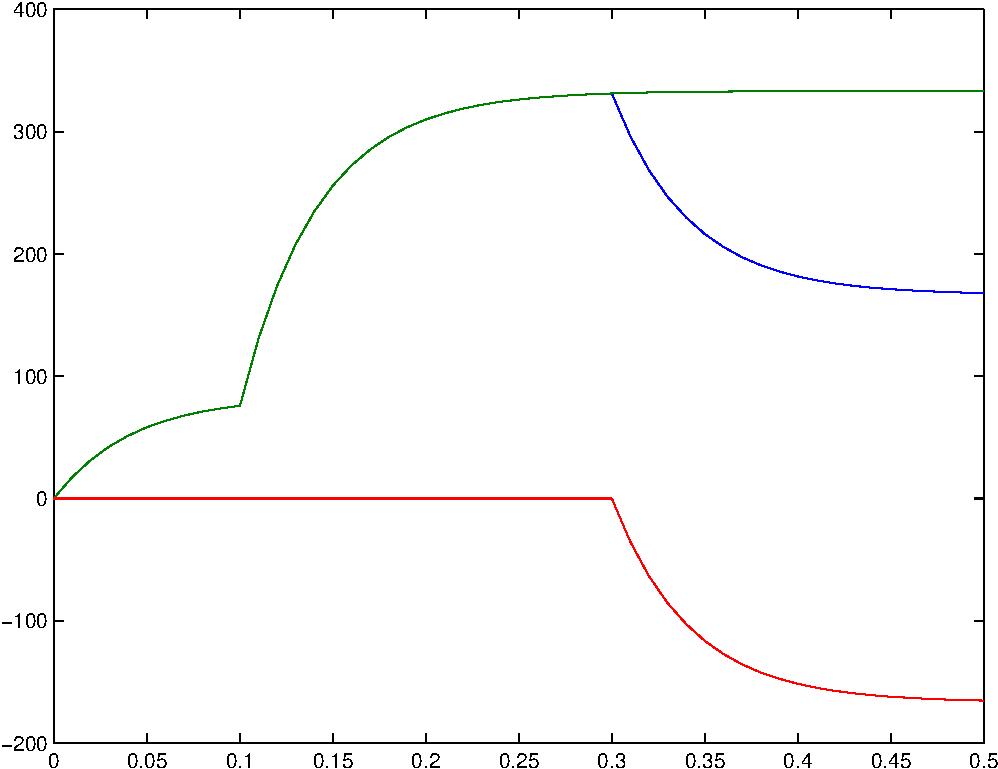
\includegraphics[width=0.6\textwidth]{03/transfer_plot.pdf}
    \caption{Simulationsergebnis}
    \label{fig:03plot}
\end{figure}
